\chapter{Additive Network Integration (A + N + I)}\label{chap:4}

\begin{figure}[H]
    \centering
    
\includegraphics[width=1\linewidth]{figures/chapter 4/ch4_ANI.pdf}
    \caption{Schematic overview of the Additive Network Integration (ANI) strategy used in the HANI scaffold platform. The figure illustrates the progressive integration of anisotropic polycaprolactone (PCL) architectures—including aligned, circumferential, and thermomolded grids—into gelatin-based hydrogels. These additive-manufactured reinforcement networks enable tunable biomechanical properties and are engineered for seamless integration within the hydrogel matrix to mimic native meniscal anisotropy.}
    \label{fig:ch4_ANI}
\end{figure}

\section{Additive Network Integration (A + N + I)}

Effective meniscal tissue engineering demands more than biocompatibility—it requires constructs that can reproduce the meniscus's complex mechanical behavior while supporting integration into the host environment. While hydrogel-based scaffolds offer excellent biological compatibility and hydration properties, their intrinsic mechanical limitations have hindered translation to load-bearing applications. Specifically, gelatin-based hydrogels, though useful for cell encapsulation and biochemical mimicry, exhibit poor resistance to the tensile and compressive forces encountered in vivo.

To address these limitations, additive manufacturing (AM) technologies provide a transformative path forward. Bioprinting offers unprecedented control over scaffold architecture, enabling fabrication strategies that bridge the gap between biological compatibility and mechanical function. The Additive Network Integration (A + N + I) approach—central to the HANI platform—leverages these AM capabilities to embed reinforcing fiber networks directly within hydrogel matrices, enhancing structural integrity while maintaining modularity and scalability.

Among the most accessible and cost-effective of these technologies is Fused Deposition Modeling (FDM), which is utilized to fabricate polycaprolactone (PCL) networks with tunable geometries. PCL's favorable tensile properties, biodegradability, and ease of extrusion make it a strategic reinforcement material for hybrid scaffolds. Through FDM, grid-like and circumferential architectures can be precisely fabricated to replicate the hierarchical anisotropy of native meniscal collagen fibers—enabling mechanical performance that hydrogel-only constructs cannot achieve.

\begin{figure}[H]
    \centering
    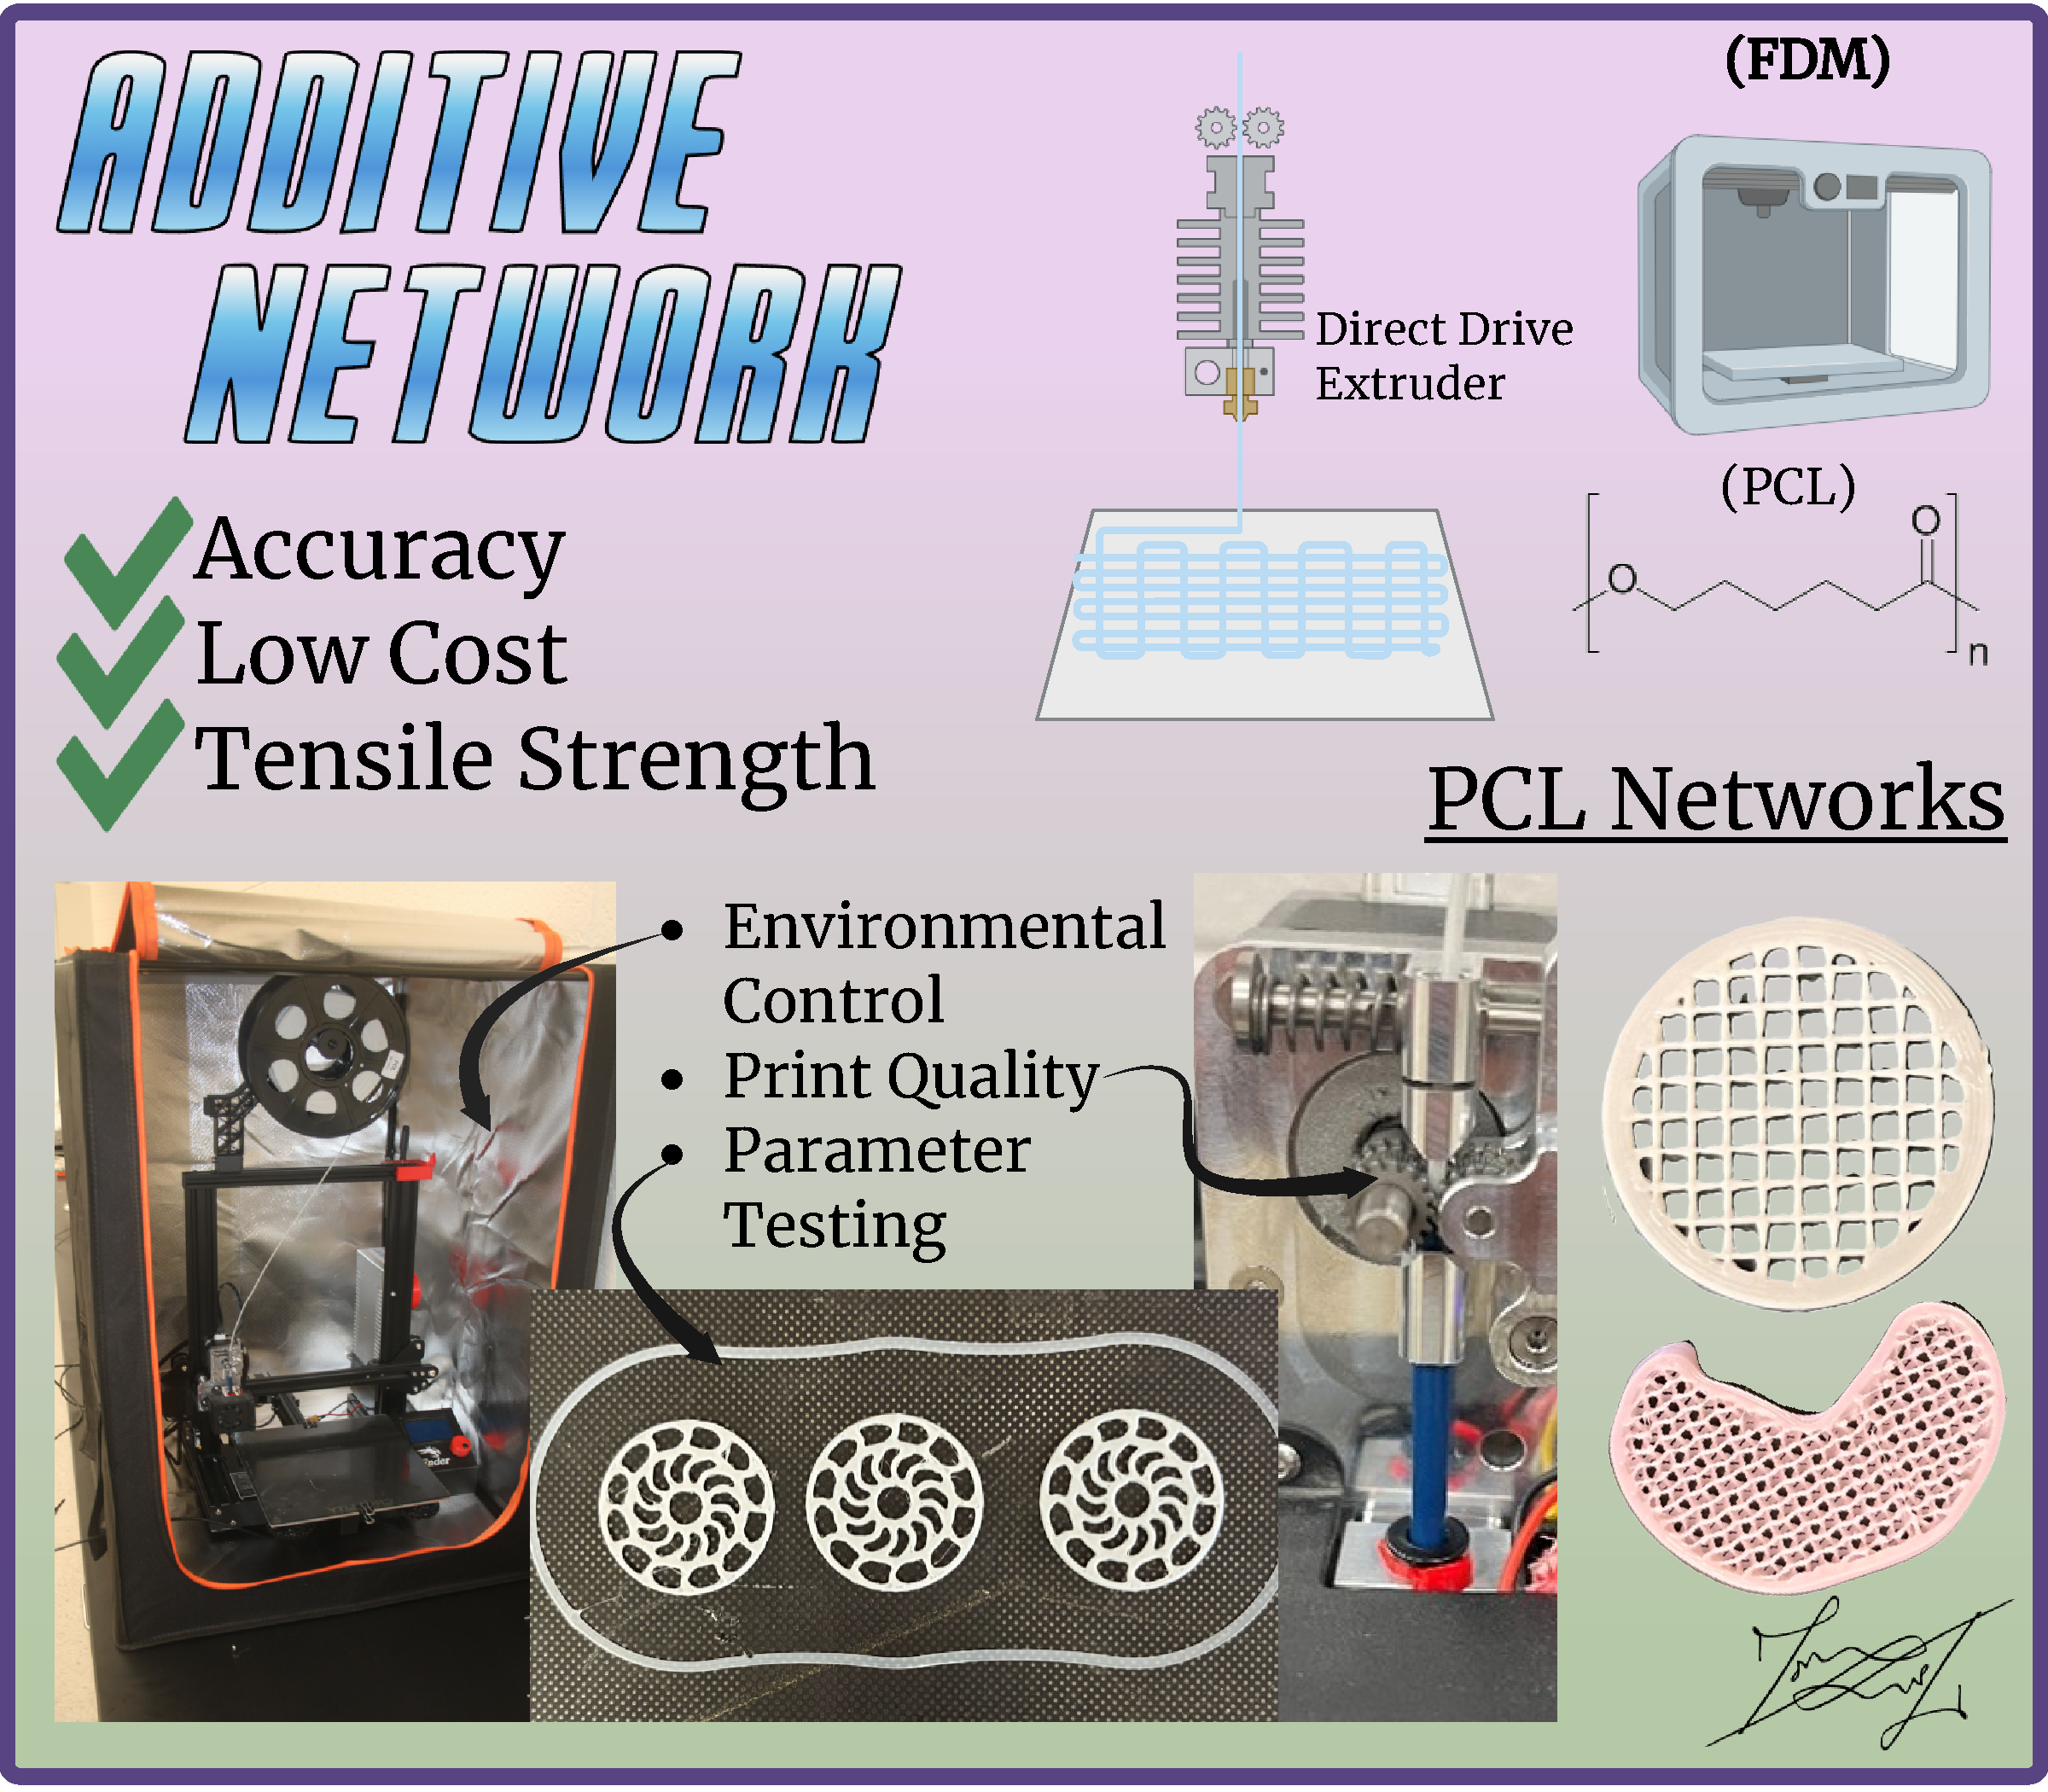
\includegraphics[width=1\linewidth]{figures/chapter 4/ch4_AN_FDM.pdf}
    \caption{Overview of polycaprolactone (PCL) network fabrication using Fused Deposition Modeling (FDM) with a direct drive extrusion system. This additive network strategy prioritizes accuracy, low cost, and enhanced tensile strength. The system features environmental control and parameter testing to optimize print quality. Representative PCL constructs, shown at bottom and right, demonstrate diverse grid and circumferential reinforcement geometries tailored for integration into hybrid hydrogel scaffolds within the HANI platform.}
    \label{fig:ch4_AN_FDM}
\end{figure}

In tandem with FDM-based PCL reinforcement, stereolithography (SLA) introduces new possibilities for high-resolution mold and scaffold component fabrication. SLA provides exceptional surface finish and dimensional fidelity, supporting the creation of intricate features that are critical for guided network integration and hydrogel shaping. By using SLA to fabricate 3D thermomolds, thermal masks, and scaffold-specific alignment guides, the A + N + I platform can achieve precise interfacial bonding and spatial organization of the composite components.

SLA’s compatibility with photoinitiated crosslinking chemistries also facilitates various mold geometry for integration of hydrogels and printed structures, reinforcing construct cohesion without compromising material properties. Moreover, the ability to rapidly prototype molds and support structures allows for patient-specific customization and iterative design testing, greatly enhancing translational potential.

\begin{figure}[H]
    \centering
    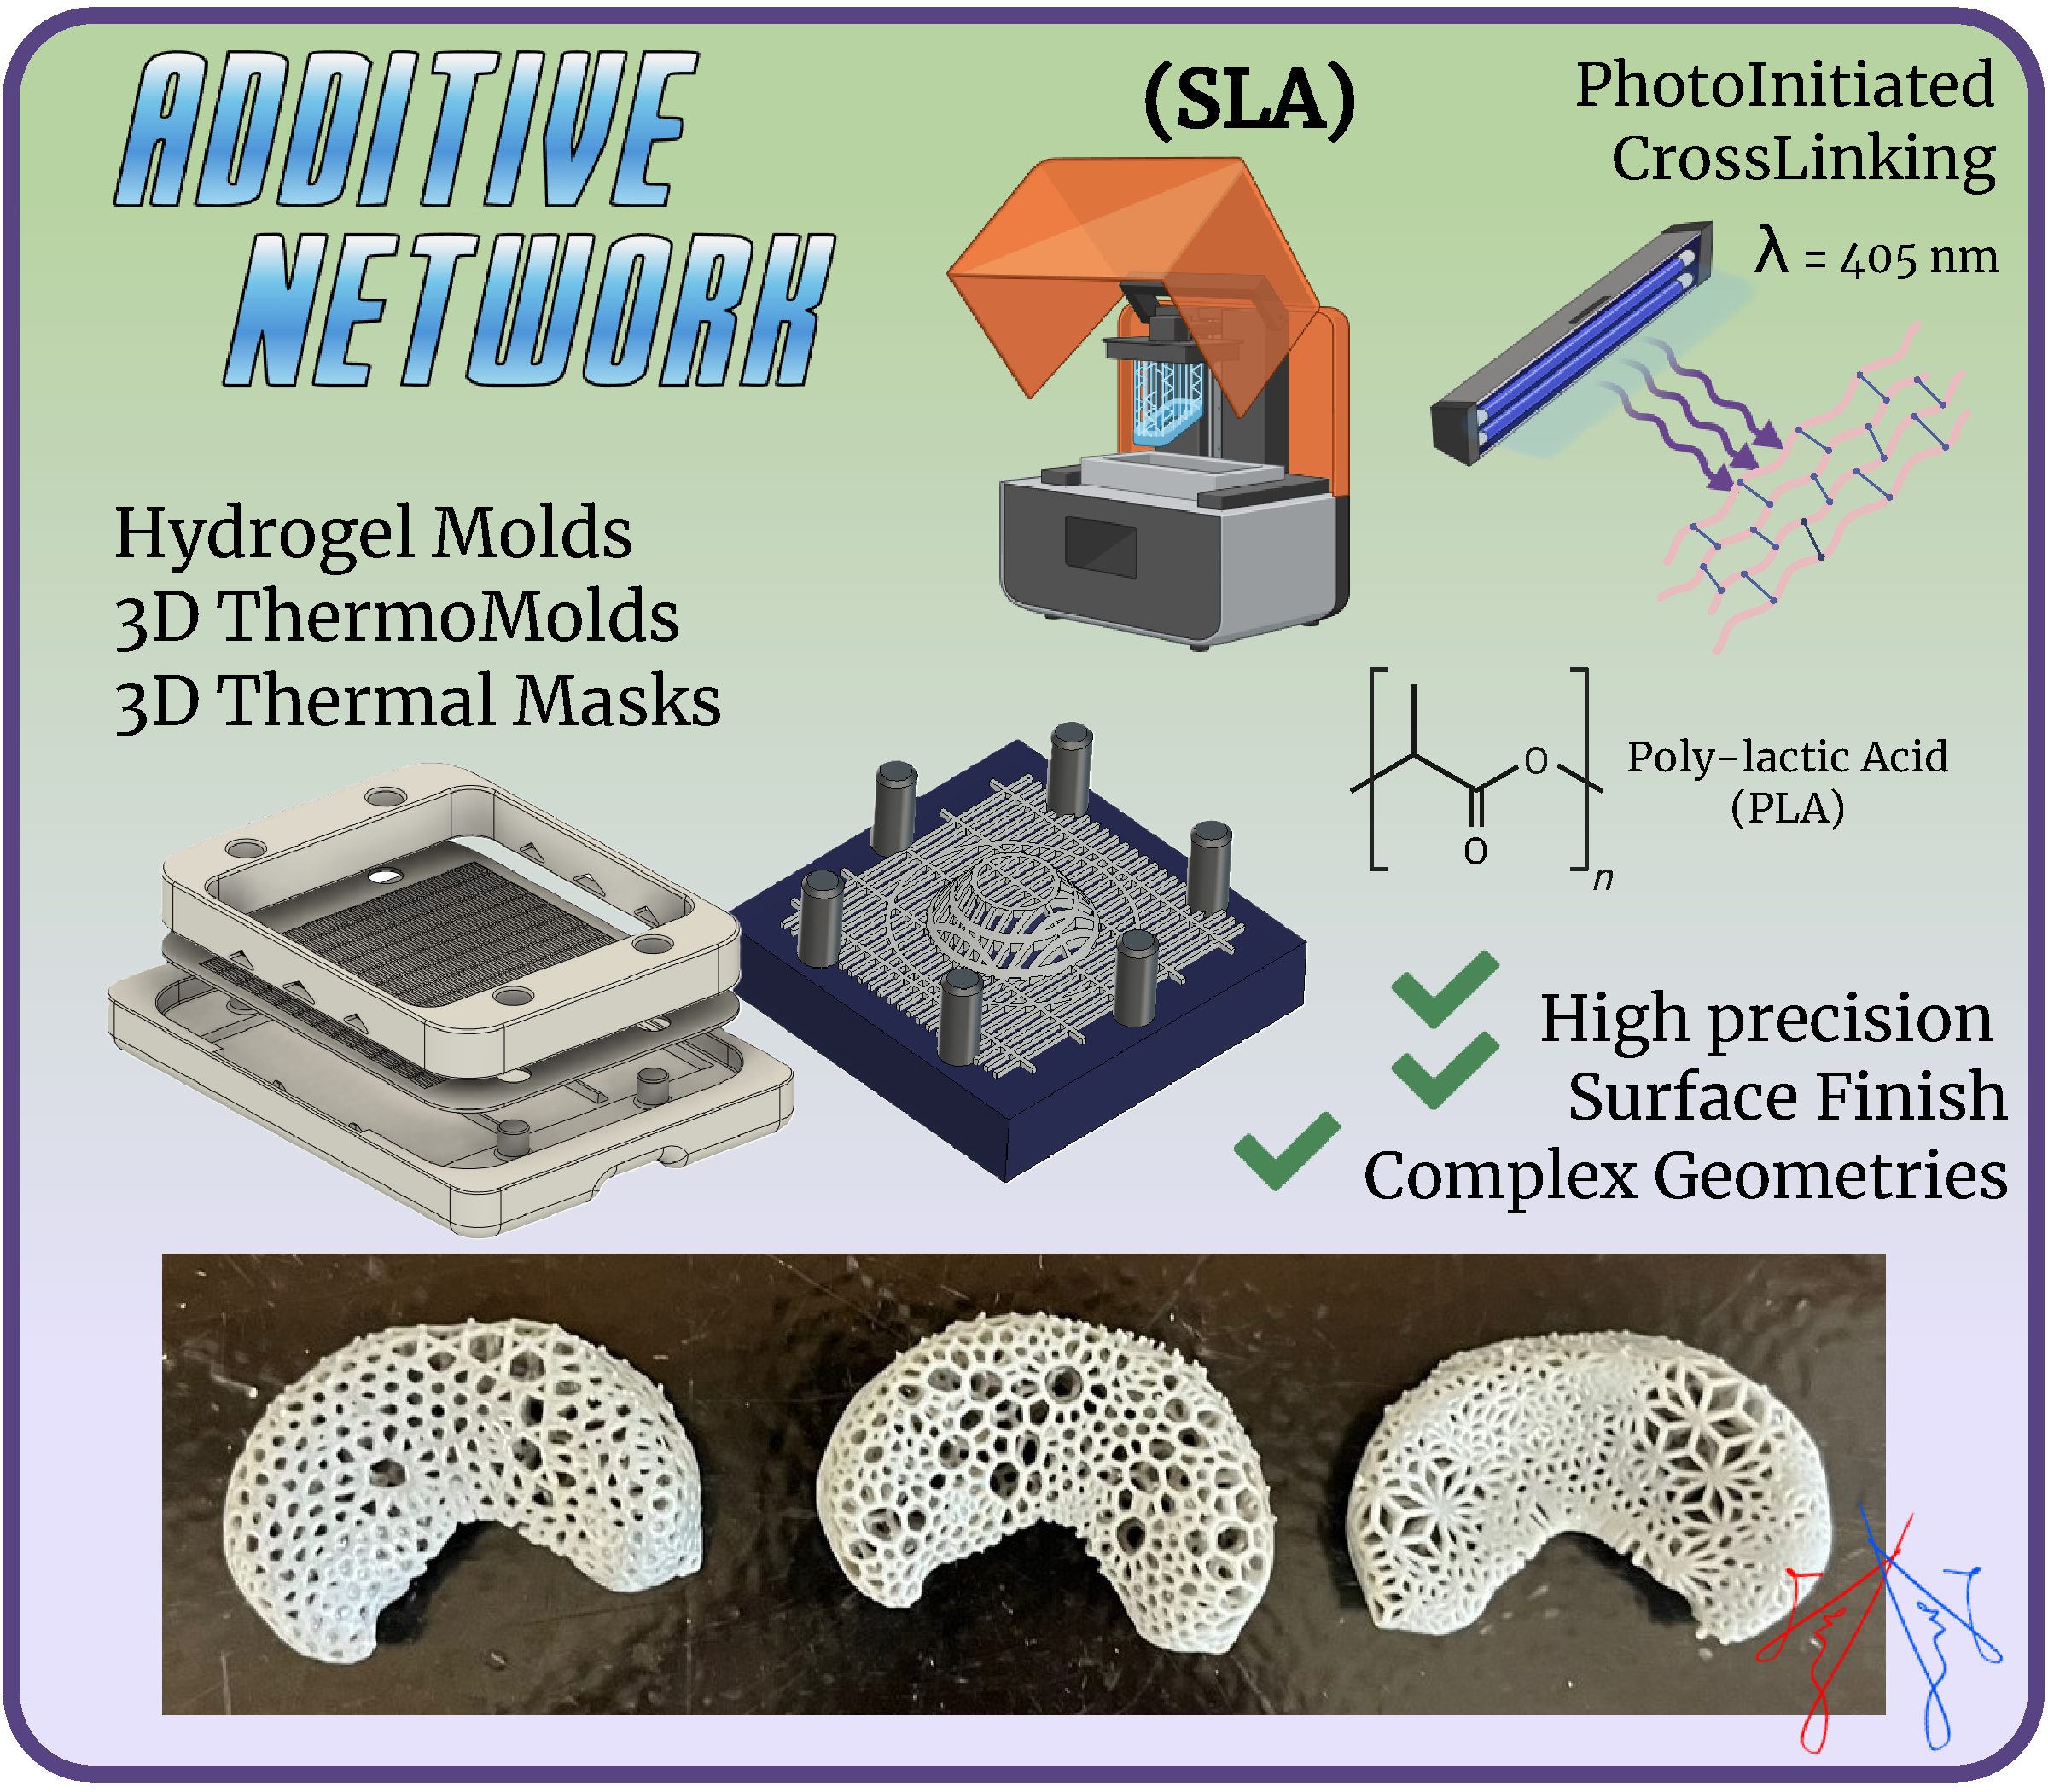
\includegraphics[width=1\linewidth]{figures/chapter 4/ch4_AN_SLA.pdf}
    \caption{Illustration of the Additive Network fabrication approach utilizing stereolithography (SLA) and photoinitiated crosslinking for scaffold design. Custom-designed hydrogel molds, 3D thermomolds, and thermal masks enable fabrication of complex geometries with high surface fidelity. The integration of poly-lactic acid (PLA) networks allows for precision-molded reinforcement elements, while ultraviolet light ($\lambda$ = 405 nm) initiates crosslinking reactions. Bottom panel: SLA-fabricated meniscus-shaped networks exhibiting high porosity and spatial accuracy for composite scaffold reinforcement.}
    \label{fig:ch4_AN_SLA}
    \end{figure}

Altogether, the A + N + I methodology capitalizes on the strengths of both FDM and SLA to create mechanically competent, biologically integrated scaffolds for meniscal repair. Through a modular and iterative engineering workflow, these technologies allow for rapid innovation in scaffold design—advancing the clinical readiness of next-generation meniscal replacements.

\subsection{Evolution of Network Integration in Tissue Engineering}

The development of functional meniscal scaffolds requires more than biochemical compatibility—it hinges on the ability to replicate the native tissue’s complex mechanical architecture. Traditional reinforcement strategies in soft tissue engineering, such as random fiber meshes or embedded textiles, have offered limited success in mimicking the anisotropic and load-bearing nature of the meniscus. These early approaches lacked spatial precision, leading to poor reinforcement integration, mechanical inconsistency, and insufficient guidance for cellular infiltration or matrix organization.

A key limitation in past scaffold designs has been the inability to precisely control the geometry, alignment, and positioning of reinforcement elements. Conventional fabrication techniques—including freeze-drying, salt-leaching, and solvent casting—lack the resolution and tunability needed to replicate the hierarchical microstructures found in native connective tissues. Consequently, many scaffolds have failed to balance mechanical integrity with biological function, impeding their translational potential.

Additive manufacturing (AM) technologies offer a compelling solution to these challenges by enabling spatially resolved, digitally guided fabrication of scaffold components. In particular, fused deposition modeling (FDM) and stereolithography (SLA) have become vital tools in regenerative scaffold design. FDM allows for the extrusion of polycaprolactone (PCL) networks with customizable fiber orientation, density, and pattern complexity. SLA complements this capability by enabling high-resolution fabrication of hydrogel molds, thermal masks, and other integration components with exceptional surface finish and structural fidelity.

The Additive Network Integration (ANI) workflow developed in this study leverages the synergistic strengths of both FDM and SLA to produce hybrid scaffolds that combine mechanical reinforcement with biological adaptability. The methodology follows a modular, iterative pipeline:  
(1) design and simulation of network architectures using CAD tools;  
(2) fabrication of PCL grids using FDM with tunable print parameters;  
(3) SLA-based mold development for hydrogel shaping and alignment; and  
(4) integration of the components within a gelatin-based matrix crosslinked under photoinitiated or thermal conditions.  

This systematic framework enables precise control over the positioning, bonding, and mechanical engagement of the reinforcing network with the hydrogel bulk, addressing long-standing issues of structural mismatch and mechanical failure seen in previous scaffold designs.

As shown in Figure~\ref{fig:ch4_ANI_flow}, this integrative approach allows us to tailor scaffold architecture across multiple scales, offering a versatile platform for meniscal tissue engineering and potentially other load-bearing orthopedic applications.

\begin{figure}[H]
    \centering
    
\includegraphics[width=1\linewidth]{figures/chapter 4/ch4_ANI_flow.pdf}
    \caption{Workflow schematic illustrating the Additive Network Integration (A + N + I) strategy within the HANI platform. The flow highlights the evolution of scaffold design from early unreinforced hydrogels to hybrid constructs incorporating anisotropic polycaprolactone (PCL) networks via additive manufacturing. By combining fused deposition modeling (FDM) and stereolithography (SLA), the A + N + I approach enables spatially controlled reinforcement integration, enhanced mechanical performance, and scaffold architectures tailored to mimic the complex structural anisotropy of native meniscal tissue.}
    \label{fig:ch4_ANI_flow}
\end{figure}

\subsection{Illustrative Overview of the Additive Network Integration Process}
Figure~\ref{fig:ch4_ANI_flow} presents a comprehensive visual summary of the Additive Network Integration (ANI) workflow as developed in this study. This diagram captures the thermomechanical and fabrication steps used to integrate polycaprolactone (PCL) reinforcement networks within a gelatin-based hydrogel matrix, culminating in the production of a hybrid HANI scaffold. The process unfolds sequentially along the illustrated purple path, guiding the viewer through each phase of scaffold development from alignment to final sample extraction.

The process begins in the top-central region of the figure, where alignment and positional accuracy are established using a custom mold equipped with vertical guide pins. These fixtures ensure reproducible placement of the PCL network and minimize dimensional deviations prior to thermal processing. Once the network is secured, controlled thermal molding is initiated using a directed heat source (indicated by the sun icon at 60°C), softening the PCL structure and allowing it to conform to the intended anatomical curvature within the mold cavity.

Following this initial shaping step, the structure is cooled to preserve the conformed geometry. The guide pins are removed, and the network is carefully extracted and inverted for continued processing. A thermal mask is then applied—a key innovation designed to deliver localized heating while preserving alignment and structural fidelity during hydrogel integration. This mask enables precise control over temperature gradients and material flow during composite formation.

At this stage, a heated solution of gelatin and glutaraldehyde (GelA–GTA) is introduced into the mold to encapsulate the thermally molded PCL architecture. Stirring and brief cooling ensure homogeneous gel consistency and controlled crosslinking kinetics. The thermal mask is subsequently removed, and the scaffold is allowed to crosslink over time (represented by the hourglass icon), forming a stable hybrid construct.

The final steps include demolding the construct, submerging it in aqueous solution to remove any residual chemicals or unreacted crosslinker, and mechanically punching the sample into its final cylindrical form. The lower left corner of the schematic depicts a representative HANI scaffold following full integration—demonstrating successful preservation of fiber orientation, geometric fidelity, and scaffold integrity.

This visual workflow encapsulates the core principles of the ANI methodology: modularity, precision, thermal control, and architectural reproducibility—each of which plays a vital role in engineering structurally competent meniscal scaffolds for load-bearing applications.

\subsection{Meniscal Tissue Properties and Integration Strategy}

The meniscus is a fibrocartilaginous structure that plays a critical role in knee joint biomechanics, contributing to load transmission, shock absorption, joint stability, and lubrication. Its ability to sustain and distribute complex mechanical loads stems from its highly organized, anisotropic microstructure. The circumferential collagen fibers bear the majority of hoop stresses generated during compression, while radial tie fibers prevent longitudinal splitting and contribute to overall structural cohesion. This composite architecture creates regional variations in mechanical properties, with distinct zones—outer (vascularized), middle (transitional), and inner (avascular)—exhibiting differing levels of stiffness, porosity, and cellularity.

Successfully replicating these biomechanical functions in an engineered scaffold requires a nuanced understanding of the meniscus's native architecture and an interdisciplinary strategy for structural biomimicry. Central to this effort is the recreation of the tissue’s anisotropic load distribution, achieved by embedding aligned PCL fiber networks that mimic the orientation and mechanical role of native collagen bundles. These aligned networks not only enhance tensile strength along the circumferential axis but also provide pathways for mechanical interlocking with the surrounding hydrogel matrix.

In addition to anisotropy, regional stiffness gradients must be considered to replicate the mechanical heterogeneity of the meniscus. This involves tuning the density and arrangement of PCL reinforcement within specific scaffold regions to mirror native tissue properties—ensuring that peripheral regions exhibit greater stiffness, while inner zones remain compliant to facilitate nutrient diffusion and cell infiltration.

Design objectives for biomimetic function extend beyond mechanical performance alone. Scaffold architecture must promote cellular alignment and migration, guide extracellular matrix deposition, and allow for progressive remodeling by host tissue. To achieve these goals, the integration strategy employs a combination of material science "Hybrid Hydrogel" (PCL and gelatin hydrogels), precision engineering "Augmented vis Additive" (additive manufacturing and mold design), and process optimization "Additive Network Integration"( reinforcement production and interface engineering).

Collectively, this interdisciplinary approach aims to construct a scaffold system that is not only mechanically robust and biomimetic but also scalable and adaptable to patient-specific geometries. Through iterative design and rigorous validation, the strategy ensures that each scaffold iteration moves closer to replicating the multifaceted roles of the native meniscus in vivo.

\begin{figure}[H]
    \centering
    
\includegraphics[width=1\linewidth]{figures/chapter 4/ch4_ANI_firstGen.pdf}
    \caption{First-generation development of the Additive Network Integration (ANI) platform. Early attempts at embedding PCL grids within hydrogel matrices faced challenges related to vertical displacement and poor alignment. Mold designs were progressively refined through the addition of internal supports and reinforcement features, ultimately enabling controlled gelatin delivery and improved integration of aligned fiber architectures.}
    \label{fig:ch4_ANI_firstGen}
\end{figure}

\subsection{First Generation: Basic Aligned Networks}

The foundational phase of Additive Network Integration (ANI) development focused on fabricating basic aligned PCL fiber networks designed to replicate the circumferential collagen alignment of native meniscal tissue. These early constructs were developed using standard CAD software and printed via fused deposition modeling (FDM) in a linear grid configuration, serving as a proof-of-concept for fiber alignment and hydrogel compatibility.

Fabrication parameters were systematically varied to achieve consistent network geometry. PCL filaments were printed with thicknesses between 0.2--0.6~mm, layer heights from 100--300~$\mu$m, and nozzle temperatures ranging from 120--140$^\circ$C. Print speeds of 10--30~mm/s were tested, with slower rates yielding improved fiber uniformity. A heated bed maintained at 30--35$^\circ$C enhanced adhesion and minimized cooling-related distortion.

Initial prototypes exposed several limitations, including uncontrolled vertical displacement of the PCL network during casting, poor adhesion, fiber warping, and uneven hydrogel crosslinking. These issues led to multiple design refinements: mold geometry was improved with internal supports to restrict vertical shift, adhesive sprays enhanced bed adhesion, and thermal profiles were tuned for post-print stability. Gelatin delivery was redirected through peripheral mold channels to ensure uniform infiltration with minimal network disturbance.

Despite its limitations, the first-generation ANI scaffold established core design principles in thermal management, structural stabilization, and hydrogel integration. These insights directly informed the development of more advanced architectures and integration strategies realized in later stages of the HANI platform.

\begin{figure}[H]
    \centering
    
\includegraphics[width=1\linewidth]{figures/chapter 4/ch4_ANI_secondGen.pdf}
    \caption{Schematic and physical representations of the second-generation Additive Network Integration (ANI) constructs featuring circumferential reinforcement. Top left: CAD rendering of the circumferential fiber grid. Middle and bottom panels: printed PCL networks, mold redesigns incorporating central standoffs and venting systems, and 3D integration of curved meniscal geometries. These adaptations were essential to preventing vertical fiber displacement, improving hydrogel flow, and enabling load-responsive network distribution.}
    \label{fig:ch4_ANI_secondGen}
\end{figure}

\subsection{Second Generation: Circumferential Reinforcement}

The second generation of Additive Network Integration (ANI) scaffolds introduced several structural and procedural innovations aimed at improving mechanical performance, spatial fidelity, and hydrogel integration. Advancing beyond the linear alignment strategies of the first generation, this iteration incorporated circumferential fiber bands into the PCL network architecture to better emulate the hoop stress-resisting capacity of native meniscal tissue. These bands played a crucial role in transforming axial compressive forces into circumferential tensile stresses—a hallmark of meniscal biomechanics. To further improve dimensional control and suppress geometric distortion during gelatin infusion, secondary transverse support bands were added. These elements helped maintain flatness and in-plane alignment, reducing fiber sagging and displacement, particularly during thermal and hydrogel-processing stages.

To support uniform hydrogel integration, a mold-based gelatin delivery system was developed. Custom ports embedded along the mold periphery enabled controlled injection of the gelatin solution, promoting even dispersion and minimizing disruption of the underlying PCL network. Mold venting channels and integrated standoffs were also refined to facilitate smooth matrix flow and prevent void formation. Together, these features improved casting uniformity and scaffold integrity, ensuring more reproducible outcomes across batches.

Realizing the architectural complexity of this scaffold generation required extensive G-code customization to control fiber curvature, spacing, and wall thickness—producing constructs that more closely mirrored native tissue architecture. Concurrently, thermal processing protocols were fine-tuned by adjusting cooling rates and enclosure temperatures to preserve dimensional fidelity. Surface treatments, such as plasma activation and micro-texturing, were evaluated to strengthen PCL-hydrogel bonding and minimize phase separation. Collectively, these innovations yielded notable improvements in scaffold biomimicry, mechanical resilience, and integration reliability, setting the stage for the thermally conformed, three-dimensional constructs introduced in the third generation of the HANI platform.
 
\begin{figure}[H]
    \centering
    
\includegraphics[width=1\linewidth]{figures/chapter 4/ch4_ANI_thirdGen.pdf}
    \caption{Fabrication and integration of third-generation 3D thermomolded PCL networks using the Additive Network Integration (ANI) platform. Top row: 3D-printed circumferential-aligned PCL grids and alignment into a modular SLA-fabricated mold for thermoforming and gelatin infusion. Middle row: gelatin embedding with visible mold alignment pins and post-infusion construct stabilization. Bottom row: representative demolded scaffolds demonstrating uniform 3D curvature and high spatial fidelity, including a final hydrated hybrid construct.}
    \label{fig:ch4_ANI_thirdGen}
\end{figure}

\subsection{Third Generation: 3D Thermomolded Networks}

The third-generation evolution of the Additive Network Integration (ANI) platform introduced fully three-dimensional (3D) thermomolded PCL networks, representing a pivotal advancement in scaffold complexity and functionality. This design iteration moved beyond planar architectures by incorporating through-thickness reinforcement layers, enabling multidirectional load resistance and improved biomimicry of the hierarchical fibrous structure of the native meniscus.

At the core of this generation was the integration of a thermoforming step post-FDM printing. PCL networks, composed of both aligned and circumferential geometries, were subjected to controlled heating in custom SLA-fabricated molds designed to impart anatomical curvature. Thermoforming was performed within the polymer’s softening range (55--65$^\circ$C), allowing for malleability without compromising the structural integrity of the network. This enabled faithful conformation to native tissue curvature while preserving inter-fiber continuity.

Mechanical stability during thermoforming and hydrogel embedding was reinforced with the addition of structural features such as dowel pins, alignment standoffs, and support ribs. These elements minimized geometric deformation, prevented network collapse, and ensured reproducibility during mold assembly and crosslinking. The mold system itself was significantly redesigned to accommodate the added complexity of the 3D architectures. Modular components included embedded guide pins, anatomical contouring, and revised boundary locks for consistent sealing.

A key advancement in this generation was the introduction of a **sacrificial outer layer**, which dramatically improved post-crosslinking removal. Following thermal shaping and gelatin crosslinking, the dowel pins were removed to release vertical constraints, and the sacrificial top mold was detached, providing unobstructed access to the base of the hydrogel composite. This allowed the entire scaffold to be lifted from the bottom—eliminating shear-induced damage and preserving sample integrity. This innovation significantly improved yield, construct uniformity, and downstream handling, ensuring scalability for extended testing and replication.

In parallel, the original central gel delivery manifold was removed to accommodate the 3D thermal mask and its associated geometry. In its place, a new **peripheral gel introduction system** was developed. This outer perimeter infusion strategy allowed for controlled delivery of both the gelatin solution and glutaraldehyde crosslinker, ensuring even matrix infiltration without compromising network alignment or creating internal voids.

Together, these advancements enabled the fabrication of anatomically shaped, mechanically robust scaffolds with high spatial fidelity and integrated 3D reinforcement. The third-generation constructs demonstrated the most complete approximation of native meniscal structure to date, positioning the platform for advanced biomechanical evaluation and preclinical translational testing.

\subsection{Mold Design Evolution}

The evolution of mold design was pivotal in enabling precise alignment, secure placement, and reliable stabilization of the PCL reinforcement networks within the hydrogel matrix. Early prototypes utilized basic two-part mold assemblies that, although functional for proof-of-concept experiments, presented several challenges including poor sealing, dimensional variability, and high rates of scaffold damage during demolding.

To address these limitations, successive design iterations introduced key engineering features aimed at improving accuracy, repeatability, and user workflow. One major innovation was the incorporation of dowel pins, which provided rigid alignment of the mold components and ensured reproducible spatial registration of the PCL networks within the hydrogel casting volume. These alignment posts minimized lateral drift during assembly and molding, preserving fiber orientation and geometric fidelity throughout the integration process.

Further advancements included the implementation of a dual-component top mold system. This configuration enabled demolding in a staged manner: once crosslinking was complete, the top mold layer could be removed independently, exposing the gelled construct while maintaining structural support from the bottom mold. Following this, the dowel pins were withdrawn, releasing the scaffold without the application of disruptive shear forces.

Another critical development was the addition of a sacrificial outer zone around the scaffold cavity. This peripheral region acted as a buffer to absorb mechanical stresses during demolding and allowed for the scaffold to be extracted from below without direct contact to the reinforced architecture. This modification drastically reduced damage rates and increased fabrication consistency, especially in thermomolded 3D scaffolds.

Together, these mold refinements resulted in a robust, modular system capable of supporting complex scaffold architectures while enabling streamlined demolding and improved production throughput. These enhancements established a reproducible platform that could be scaled for both experimental and translational scaffold fabrication.

\subsection{Integration Engineering}

Effective integration of the PCL reinforcement networks within the gelatin hydrogel matrix was essential for achieving mechanically coherent, structurally stable scaffolds. In the HANI platform, integration was achieved through physical encapsulation rather than chemical bonding, requiring tight control over hydrogel handling, crosslinking kinetics, and thermal conditions during fabrication.

Initial integration methods using a central gelatin delivery manifold proved incompatible with the addition of a 3D thermal mask, which occupied the central mold cavity. As a result, a new peripheral gel introduction strategy was developed. Gelatin and glutaraldehyde (GTA) were infused around the mold perimeter via distributed entry points, allowing for more uniform hydrogel infiltration without disturbing the thermomolded network geometry.

Precise control over gelatin introduction was critical to prevent the formation of voids, air bubbles, or incomplete encapsulation zones. Gelatin was introduced slowly and incrementally, allowing it to fully flow around and beneath the PCL network. This approach ensured that the hydrogel matrix surrounded the entire fiber structure, maximizing mechanical interlock and stabilizing the composite architecture.

Equally important was the regulation of GTA crosslinking. The crosslinker was titrated gradually to ensure even diffusion and uniform gelation. Rapid or localized crosslinking was avoided to prevent stiff regions or inconsistent bonding at the PCL-hydrogel interface. This stepwise infusion approach produced constructs with consistent mechanical properties and cohesive internal structure.

Throughout the integration process, thermal conditions were closely monitored using infrared (IR) thermometry. Gelatin temperature was maintained within an optimal working range (~40--45$^\circ$C) to ensure flowability while avoiding denaturation. Simultaneously, care was taken to prevent overheating of the PCL network, which could result in warping or fiber misalignment. The interplay of thermal control, fluid handling, and crosslinking kinetics was essential to preserving scaffold geometry and achieving a well-integrated final construct.

In summary, the integration engineering strategy was built around precise thermal and fluidic control, a redesigned gel delivery system, and gradual crosslinking. These elements worked synergistically to embed the PCL networks within the hydrogel matrix in a consistent, reproducible manner—meeting the structural demands of meniscal tissue engineering applications.

\subsection{Quality Metrics and Reproducibility}

Ensuring reproducibility and process reliability was a central focus in the development of the HANI scaffold fabrication workflow. To support scalability and downstream translation, production quality was continuously monitored across multiple fabrication cycles, with attention to both process parameters and resulting scaffold characteristics.

Dimensional consistency and structural fidelity were qualitatively assessed by comparing fabricated scaffolds to their original CAD specifications. Observations of fiber alignment, pore pattern uniformity, and overall scaffold shape were used to confirm that the combined use of fused deposition modeling (FDM) and SLA-based molding yielded constructs with high conformity to design intent.

To assess batch reproducibility, multiple scaffold sets were fabricated under standardized conditions. Throughout this process, sample quality was evaluated with regard to geometric consistency, integration of the PCL networks, and visual inspection for defects such as delamination, voids, or incomplete embedding. These checks confirmed the stability of the mold design and the reliability of the integration procedure.

Critical parameters—including print settings, thermal profiles, gelatin introduction methods, and crosslinking conditions—were carefully monitored to identify sources of variation. Observed deviations were tracked and used to inform iterative refinements to the workflow, supporting a feedback loop that prioritized both quality control and fabrication efficiency.

Taken together, these quality monitoring practices established a reproducible and scalable fabrication protocol. The combination of design verification, batch inspection, and process oversight ensured consistent scaffold production, reinforcing the platform’s suitability for further preclinical development and translational application.

\section{Scale-Up Considerations}

As the scaffold fabrication process advanced toward translational relevance, comprehensive scale-up considerations were evaluated to ensure the system’s feasibility for both research and clinical applications. This section addresses customization potential, manufacturing scalability, equipment and materials cost analysis, and regulatory pathways.

\subsection{Customization and Patient-Specific Adaptation}

A primary focus of the scale-up process was assessing the adaptability of the scaffold system for patient-specific production. The modular mold design, combined with the flexibility of additive manufacturing, allows rapid customization of scaffold geometries based on medical imaging data such as MRI or CT scans. This capability enables the production of anatomically accurate constructs tailored to individual patient anatomy, a key factor for clinical translation in orthopaedic tissue engineering.

\subsection{Manufacturing Scalability}

High-throughput production strategies were explored to assess scalability. The fabrication process demonstrated compatibility with affordable desktop-scale 3D printers, allowing multiple scaffolds to be manufactured simultaneously with minimal specialized infrastructure. Batch processing protocols and optimized mold assembly methods further enhanced throughput, creating a practical foundation for automated and semi-automated production systems. 

Feasibility studies confirmed that the process can be reliably replicated across multiple workstations, supporting decentralized manufacturing models such as point-of-care scaffold fabrication within clinical settings. This approach reduces lead times and supports just-in-time production workflows, aligning with modern clinical needs.

\subsection{Equipment and Materials Cost Analysis}

A cost-effective setup is essential for both research scalability and potential clinical translation. The scaffold fabrication process utilized two primary 3D printer models:

\begin{itemize}
    \item \textbf{Creality Ender 3 Series (FDM):} This widely adopted printer offers a cost-effective solution for fabricating PCL reinforcement networks. The Creality Ender 3 V3 SE, for example, is priced at approximately \$199 USD \cite{creality_ender3}.
    
    \item \textbf{ELEGOO Saturn 4 Ultra (SLA):} Suitable for high-resolution mold fabrication, this resin printer is priced at around \$399 USD \cite{elegoo_saturn4}.
\end{itemize}

The materials used in scaffold production include:

\begin{itemize}
    \item \textbf{Polycaprolactone (PCL):} A biodegradable polyester forming the scaffold’s reinforcing network. Research-grade PCL is available at prices ranging from \$15 to \$80 per kilogram, depending on purity and supplier \cite{pcl_price}.
    
    \item \textbf{Gelatin Type A:} Derived from porcine skin, this forms the hydrogel matrix. Research-grade gelatin Type A costs approximately \$20 per kilogram \cite{gelatin_price}.
    
    \item \textbf{Glutaraldehyde (GTA):} Used as the crosslinking agent; prices vary based on concentration and supplier.
\end{itemize}

\begin{table}[H]
\centering
\begin{tabular}{|l|l|l|}
\hline
\textbf{Item} & \textbf{Estimated Cost (USD)} & \textbf{Notes} \\
\hline
Creality Ender 3 V3 SE & \$199 & FDM printer for PCL scaffolds \\
ELEGOO Saturn 4 Ultra & \$399 & SLA printer for mold fabrication \\
Polycaprolactone (PCL) & \$15--\$80/kg & Depends on purity and supplier \\
Gelatin Type A & \$100/kg& Research-grade, porcine-derived \\
Glutaraldehyde (GTA) & Variable & Based on concentration \\
\hline
\end{tabular}
\caption{Estimated Costs of Equipment and Materials}
\end{table}

\subsection{Process Control and Quality Assurance}

Ensuring consistent scaffold quality at scale requires meticulous process control. Throughout fabrication, critical parameters such as print temperatures, gelatin introduction rates, and glutaraldehyde titration were carefully monitored. An infrared (IR) thermometer was used to continuously track the temperature of the gelatin hydrogel and PCL network, ensuring that gelatin remained within optimal processing temperatures and that PCL did not warp or deform. This real-time monitoring allowed precise control over the integration process, contributing to high reproducibility and reliable scaffold performance.

\subsection{Regulatory Compliance Pathways}

As part of translational planning, regulatory compliance pathways were also considered. Initial assessments prioritized the use of biocompatible and research-grade materials, including medical-grade PCL, and emphasized process documentation in alignment with good manufacturing practice (GMP) standards. Future work will focus on formal biocompatibility testing, sterility validation, and adherence to regulatory requirements essential for progressing toward clinical trial readiness.

\subsection{Summary}

The scaffold system demonstrated strong potential for scalable and patient-specific production. Affordable, modular equipment, combined with streamlined workflows and precise process controls, established a clear pathway for both research-scale fabrication and eventual clinical implementation.

% \bibliographystyle{plain}
% \begin{thebibliography}{9}
% \bibitem{creality_ender3}
% Creality Official Store. Ender-3 V3 SE 3D Printer. Retrieved from \url{https://store.creality.com/products/ender-3-v3-se-3d-printer}

% \bibitem{elegoo_saturn4}
% ELEGOO Official Store. Saturn 4 Ultra 12K Resin 3D Printer. Retrieved from \url{https://us.elegoo.com/products/saturn-4-ultra-12k-10inch-monochrome-lcd-resin-3d-printer}

% \bibitem{pcl_price}
% Made-in-China.com. Polycaprolactone Price. Retrieved from \url{https://www.made-in-china.com/products-search/hot-china-products/Polycaprolactone_Price.html}

% \bibitem{gelatin_price}
% Thermo Fisher Scientific. Gelatin, Type A, 175 Bloom. Retrieved from \url{https://www.thermofisher.com/order/catalog/product/J61548.A1}
% \end{thebibliography}

\section{ANI–Poroviscoelastic Characterization}

The additive network integration strategies outlined thus far have culminated in a scaffold system that exhibits advanced architectural fidelity, precise fabrication control, and consistent integration between polycaprolactone (PCL) networks and gelatin hydrogels. Through iterative refinement, including the progression from aligned grids to fully thermomolded 3D reinforcements, and the parallel evolution of mold systems and fabrication workflows, the HANI platform has matured into a robust framework for meniscal tissue engineering.

While these developments have validated the platform’s capacity for structural mimicry and reproducible fabrication, mechanical performance remains a critical dimension requiring deeper exploration. The native meniscus exhibits a complex poroviscoelastic behavior—characterized by fluid-dependent load distribution, time-dependent stress-relaxation, and dynamic creep under physiological loading. Reproducing these mechanical characteristics in engineered scaffolds is essential for long-term functionality and biological success.

The following section transitions from structural design to functional assessment, focusing on the poroviscoelastic characterization of HANI scaffolds. This includes mechanical testing protocols designed to simulate physiologic loading conditions, evaluation of stress-relaxation and time-dependent strain responses, and analysis of scaffold behavior under compressive and cyclic loading. These studies aim to elucidate the extent to which the hybrid PCL–gelatin composite mimics native tissue mechanics and to identify parameters for further optimization.

This transition marks a pivotal shift from fabrication-focused innovation to performance validation, aligning the scaffold development trajectory with clinical functional requirements. By coupling structural precision with biomechanical fidelity, the HANI platform continues its evolution toward a comprehensive solution for meniscal regeneration.
